
In the last three Chapters we have introduced six important \PETSc objects for solving PDEs:
\begin{itemize}
\item[\quad Chapter \ref{chap:ls}:] \pVec, \pMat, \pKSP, \pPC
\item[\quad Chapter \ref{chap:st}:] \pDM\sidenote{In the \pDMDA case only.}
\item[\quad Chapter \ref{chap:nl}:] \pSNES
\end{itemize}
Each example in the rest of the book will use \emph{all} of these object types.

In particular, from now on we will even solve \emph{linear} PDEs using a \pSNES object and Newton iteration.  Linear problems are now merely the case where we know, in advance, that one Newton iteration suffices.  Always using \pSNES gives us uniform code structure and much more flexibility when it comes to changing the PDE problem.

Though new ideas appear in it, the current Chapter takes a break from introducing new \PETSc objects.  Instead we look at a PDE which arises from minimization in a function space, and we introduce a structured-grid finite element method.  Our one example is from the important class of nonlinear PDEs which are Poisson-like, but with solution-dependent diffusivity.


\section{$p$-Laplacian equation as minimization}

Let $\Omega$ be a domain (connected open subset) in $\RR^2$ or $\RR^3$ with well-behaved boundary.\sidenote{A Lipschitz boundary will suffice in theory.  In practice we use polygonal domains, a rectangle in the current Chapter and general polygons in Chapter \ref{chap:un} when we return to FEMs.}  Consider this nonlinear functional for $p \ge 1$,
\begin{equation}
    I[u] = \int_\Omega \frac{1}{p} |\grad u|^p - fu.  \label{eq:of:functional}
\end{equation}
This functional is well-defined on the Sobolev space \citep{Evans2010} of integrable functions which are defined on $\Omega$ and have integrable gradient,
\begin{equation}
    W^{1,p}(\Omega) = \left\{w \,:\, \int_\Omega |w|^p < \infty \,\, \& \, \int_\Omega |\grad w|^p < \infty\right\}, \label{eq:of:sobolevdefn}
\end{equation}
which is a Banach space with norm $\|w\|_{W^{1,p}} = \left(\int_\Omega |w|^p + \int_\Omega |\grad w|^p\right)^{1/p}$.  We will assume that the function $f$ in \eqref{eq:of:functional} is at least integrable, in the sense that $f\in L^q(\Omega)$ for $q$ dual to $p$ (i.e.~ $1/p+1/q=1$), but little is lost if we just use continuous $f\in C(\Omega)$.

\begin{marginfigure}
\includegraphics[width=1.2\textwidth]{figs/minsurf} % generated by figs/minsurf.tex
\medskip
\caption{The functional $I[u]$ is analogous to the convex surface $z = \tfrac{1}{4}(x^4 + y^4) - 2x + 2y$ shown here, but with input from the $\infty$-dimensional space $W_g^{1,p}(\Omega)$ instead of the plane $\RR^2$.}
\label{fig:of:cartoonfunctional}
\end{marginfigure}

The reader may visualize $I[u]$ in \eqref{eq:of:functional} in cartoon form as in Figure \ref{fig:of:cartoonfunctional}.  As suggested by this cartoon it has a unique minimum, at least if we add boundary conditions.

We add Dirichlet conditions (Chapter \ref{chap:st}) by choosing a real-valued function $g$ defined along $\partial \Omega$.  This function determines a subset (affine subspace) of $W^{1,p}(\Omega)$, namely
\begin{equation}
    W_g^{1,p}(\Omega) = \left\{w \,:\, w \in W^{1,p}(\Omega) \,\, \& \,\, w\big|_{\partial \Omega} = g\right\},  \label{eq:of:affinedirichlet}
\end{equation}
consisting of those functions which have boundary value $g$.  For this to make sense we assume $g \in L^p(\partial \Omega)$ and note that ``$w\big|_{\partial \Omega} = g$'' has a precise ``trace operator'' meaning \citep{Evans2010}.  These considerations also define the vector subspace $W_0^{1,p}(\Omega) \subset W^{1,p}(\Omega)$ in the case where $g=0$; we use this subspace for ``test functions'' below.

The functional $I[u]$ has three significant properties.  First of all, with the Dirichlet boundary conditions, $I[u]$ is \emph{coercive} in the sense that if the input function from $W_g^{1,p}(\Omega)$ is large in norm then the output is large:
\begin{equation}
\lim_{\|u\|_{W^{1,p}} \to +\infty} I[u] = +\infty.   \label{eq:of:coercivity}
\end{equation}
Secondly it is continuous enough to have a minimum on compact sets, namely it is \emph{weakly lower semi-continuous}, which means, by definition, that
\begin{equation}
\lim_{u\rightharpoonup v} I[u] \ge I[v],  \label{eq:of:lowersemicont}
\end{equation}
where the limit is in the weak topology on $W^{1,p}(\Omega)$ \citep{Evans2010,KinderlehrerStampacchia1980}.  Third it is \emph{convex}, meaning
\begin{equation}
I[\lambda u + (1-\lambda) v] \le \lambda I[u] + (1-\lambda) I[v]    \label{eq:of:convexity}
\end{equation}
if $u,v\in W^{1,p}(\Omega)$ and $0 \le \lambda \le 1$.

\citet{KinderlehrerStampacchia1980} show that the three properties \eqref{eq:of:coercivity}, \eqref{eq:of:lowersemicont}, \eqref{eq:of:convexity} imply that the problem
\begin{equation}
\min_{u \in W_g^{1,p}(\Omega)} I[u] \label{eq:of:plapmin}
\end{equation}
has a unique solution.  Being good calculus students we immediately seek this solution by taking the derivative and setting it to zero.  Fortunately, if $p>1$ then the functional $I[u]$ is smooth enough to have a gradient (derivative).

In fact, if $p>1$ then the solution of minimization problem \eqref{eq:of:plapmin} is also the solution to a nonlinear PDE.  The statement that the gradient is zero at the minimum has several names, among them \emph{variational equation}, \emph{Euler-Lagrange equation}, and the \emph{weak form of the PDE}.  These multiple names hint that one sees the following calculation in many parts of applied mathematics.

Assume $\eps$ is a real number and $u,v \in W^{1,p}(\Omega)$.  Then
\begin{align*}
I[u+\eps v] - I[u] &= \int_\Omega \frac{1}{p} |\grad u + \eps \grad v|^p + \frac{1}{p} |\grad u|^p - \eps f v \\
   &= \eps \left(\int_\Omega |\grad u|^{p-2} \grad u \cdot \grad v - f v\right) + O(\eps^2),
\end{align*}
and so the directional derivative, and thus the gradient, exists and has this formula:
\begin{equation}
\grad I[u](v) = \lim_{\eps\to 0} \frac{I[u+\eps v] - I[u]}{\eps} = \int_\Omega |\grad u|^{p-2} \grad u \cdot \grad v - f v. \label{eq:of:plapfunctionalderivative}
\end{equation}
That is, for each $u \in W^{1,p}(\Omega)$ formula \eqref{eq:of:plapfunctionalderivative} defines a map
   $$\grad I[u] : W^{1,p}(\Omega) \to \RR.$$

If $u \in W_g^{1,p}(\Omega)$ and $v\in W_0^{1,p}(\Omega)$ then $u+\eps v\in W_g^{1,p}(\Omega)$.  Thus if $u \in W_g^{1,p}(\Omega)$ solves \eqref{eq:of:plapmin} then the above derivative calculation shows $\grad I[u](v)=0$ or
\begin{equation}
\int_\Omega |\grad u|^{p-2} \grad u \cdot \grad v - f v = 0 \label{eq:of:plapweakform}
\end{equation}
for all $v\in W_0^{1,p}(\Omega)$.  Note that the test functions $v$ must have zero boundary values in this calculation.

From now on we refer to \eqref{eq:of:plapweakform} as the \emph{weak form} of the $p$-\emph{Laplacian} equation.  If the solution $u \in W_g^{1,p}(\Omega)$ to problem \eqref{eq:of:plapmin} is actually smooth-enough to have continuous second derivatives,\sidenote{\emph{Proving} this much smoothness is possible in some cases when the domain $\Omega$ and data $f,g$ are well-behaved.  Such results, found in \citep{KinderlehrerStampacchia1980} for example, are strongly $p$-dependent, and beyond our scope here.} i.e.~$u \in C^2(\Omega)$, then we can derive the \emph{strong form} corresponding to equation \eqref{eq:of:plapweakform}.  The strong form generalizes the Poisson problem stated in Chapter \ref{chap:st}

The strong form arises here by an integration-by-parts \citep{Evans2010} of equation \eqref{eq:of:plapweakform}, which gives
    $$-\int_\Omega \Div\left(|\grad u|^{p-2} \grad u\right) v - \int_\Omega f v + \int_{\partial \Omega} v |\grad u|^{p-2} \grad u \cdot \bn = 0$$
The boundary integral is zero if $v\in W_0^{1,p}(\Omega)$.  It follows that
\begin{equation}
- \Div\left(|\grad u|^{p-2} \grad u\right) = f,
\label{eq:of:plapstrongform}
\end{equation}
which is the strong form, the traditional form of the $p$-Laplacian equation.  It reduces to Poisson equation \eqref{poissonsquare} if $p=2$.

Before proceeding to a numerical solution, the main idea of this extended diversion into theory is simple and worth summarizing:
\begin{quote}
Minimization problem \eqref{eq:of:plapmin} for functional $I[u]$ in \eqref{eq:of:functional} is equivalent to the weak form \eqref{eq:of:plapweakform}.  It becomes the strong form \eqref{eq:of:plapstrongform} in cases where the solution $u$ is smooth.  Thus the $p$-Laplacian equation \eqref{eq:of:plapstrongform}, a nonlinear Poisson equation, arises from a minimization problem.
\end{quote}


\section{Structured $Q^1$ finite elements}

We can use \PETSc to numerically solve the $p$-Laplacian equation \eqref{eq:of:plapstrongform} \emph{as a minimization problem} based only on user code that computes the functional $I[u]$ from a representation of $u \in W_g^{1,p}(\Omega)$.  In other words, once we have a finite-dimensional representation of the input $u$, all we need to implement is formula \eqref{eq:of:functional} for $I[u]$.  Such an implementation may suffice  for initial prototyping or, as we show here, it can be augmented by additional derivative-computing code.  Initially, however, we can ask \PETSc to use finite differences when it needs derivatives (gradients) in minimizing $I[u]$.

For the representation of $u$ we introduce a structured-grid finite element method (FEM) using quadrilateral elements.  The gridded unknowns, which live on the same structured grid as in Chapter \ref{chap:st}, will in this Chapter represent a function in a function space.  The resulting code will be surprisingly-similar to a finite difference solution of PDE \eqref{eq:of:plapstrongform}, despite the conceptually-distinct approach.

\begin{marginfigure}
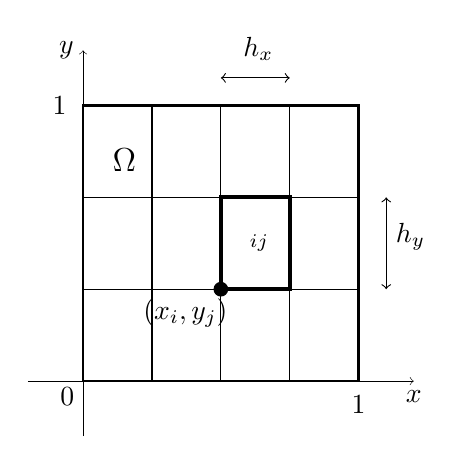
\begin{tikzpicture}[scale=3.5]
  \draw[->,very thin] (-0.2,0.0) -- (1.2,0.0) node[below] {$x$};
  \draw[->,very thin] (0.0,-0.2) -- (0.0,1.2) node[left] {$y$};
  \draw[line width=1.0pt] (0.0,0.0) -- (0.0,1.0) -- (1.0,1.0) -- (1.0,0.0) -- cycle;
  \pgfmathsetmacro\fourth{1.0/4.0}
  \pgfmathsetmacro\third{1.0/3.0}
  \pgfmathsetmacro\twothird{2.0/3.0}
  \draw[xstep=\fourth,ystep=\third,black,thin] (0.0,0.0) grid (1.0,1.0);
  % outline an element
  \draw[line width=1.5pt] (0.5,\third) -- (0.75,\third) -- (0.75,\twothird) -- (0.5,\twothird) -- cycle;
  \node at (0.64,0.5) {$\square_{ij}$};
  \filldraw (0.5,\third) circle (0.7pt) node[xshift=-4.5mm,yshift=-3mm] {$(x_i,y_j)$};
  \draw[<->] (0.5,1.1) -- (0.75,1.1) node[above,yshift=1mm,xshift=-4mm] {$h_x$};
  \draw[<->] (1.1,\third) -- (1.1,\twothird) node[right,yshift=-5mm] {$h_y$};
  \node at (0.15,0.8) {\large $\Omega$};
  \node[yshift=-3mm] at (1.0,0.0) {$1$};
  \node[xshift=-3mm] at (0.0,1.0) {$1$};
  \node[xshift=-2mm,yshift=-2mm] at (0.0,0.0) {$0$};
\end{tikzpicture}
\caption{Our domain $\Omega$ is a unit square.  The structured grid divides it into elements $\square_{ij}$ of area $h_x h_y$ indexed by their lower-left corners $(x_i,y_j)$.}
\label{fig:of:q1grid}
\end{marginfigure}

The domain is fixed to be the square $\Omega = (0,1)\times (0,1)$ in this Chapter.  Consider the structured grid on $\Omega$ shown in Figure \ref{fig:of:q1grid}.  It has nodes $(x_i,y_j)$ where $h_x=1/(m_x-1)$, $h_y=1/(m_y-1)$, $x_i = i h_x$, and $y_j = j h_y$; note $i\in \{0,1,\dots,m_x-1\}$ and $j\in\{0,1,\dots,m_y-1\}$.  The \emph{elements} are the (closed) rectangles
   $$\square_{ij} = [x_i,x_{i+1}] \times [y_j,y_{j+1}]$$
so that $\bigcup_{ij} \square_{ij} = \overline{\Omega}$ and $|\square_{ij}| = h_x h_y$.

We immediately see that the functional can be computed element-by-element, because integration is additive over sets and the boundaries are of zero measure:
\begin{equation}
I[u] = \sum_{i=0}^{m_x-1} \sum_{j=0}^{m_y-1} \int_{\square_{ij}} \frac{1}{p} |\grad u|^p - fu  \label{eq:of:sumoverelements}
\end{equation}
Integration over a single element $\square_{ij}$ can be addressed once we represent $f$ and $u$.

So, how should we approximate a function $w \in W^{1,p}(\Omega)$ in a manner compatible with the structured grid of rectangles above?  One of the simpler choices is to require that the approximation $w_h \approx w$ be bilinear on each element $\square_{ij}$ and continuous on the whole domain $\Omega$.  These requirements allow us to determine $w_h(x,y)$, for any $(x,y)\in \overline\Omega$, from the nodal values $w_{ij} = w_h(x_i,y_j)$.  In fact they determine a linear isomorphism between the vector space $\RR^N$ of possible nodal values, with $N=m_x m_y$ equal to the total number of nodes, and an $N$-dimensional linear subspace of $W^{1,p}(\Omega)$, namely
\begin{equation}
S^h = \left\{v \in C(\Omega) \, \Big| \, v|_{\square_{ij}} \text{ is bilinear}\right\}. \label{eq:of:Shdefn}
\end{equation}
Because the elements are quadrilaterals and the degree of bilinear polynomials is one, $S_h$ is a $Q^1$ \emph{finite element space} \citep{Elmanetal2005}

The solution $u$ to minimization problem \eqref{eq:of:plapmin} must, however, have the boundary values given by $g$.  If $g$ is discontinuous or if it is not piecewise-linear then its use as boundary values conflicts with the restrictions which define $S_h$.  We resolve the conflict by requiring $g$ to be well-behaved, namely continuous and (appropriately) piece-wise linear on $\partial\Omega$.  One may show in that case that the (affine) space of functions
\begin{equation}
S_g^h = \left\{v \in S_h \, \Big| \, v|_{\partial \Omega} = g\right\} \label{eq:of:Sghdefn}
\end{equation}
is an (affine) subspace of $W_g^{1,p}(\Omega)$.  Replacing $W_g^{1,p}(\Omega)$ by $S_g^h$ in problem \eqref{eq:of:plapmin} gives a \emph{conforming}\sidenote{The ``nonconforming'' version only has $u_h \approx g$ on the boundary.  For example, $u_h|_{\partial \Omega}$ might be a piecewise-linear interpolant of $g$ \citep{Elmanetal2005}.} $Q^1$ FEM in which the FEM solution $u_h\in S_g^h$ is also in $W_g^{1,p}(\Omega)$.

The next step is to describe a bilinear function on a single element $\square_{ij}$, and thereby build a basis for space $S_g^h$.  We do this by constructing bilinear functions on a \emph{reference element} $\square_\ast = [-1,1]\times[-1,1]$, in variables $\xi$ and $\eta$, as shown in Figure \ref{fig:of:q1gridandref}.\sidenote{One can avoid the reference element in the case here, in which all elements in the structured grid are congruent rectangles \citep[for example]{Bueler2015}.  However, we are thinking ahead toward less-structured examples (Chapter \ref{chap:un}).}

If $v(\xi,\eta)$ is bilinear on $\square_\ast$ then $v(\xi,\eta) = a + b\, \xi + c\, \eta + d\, \xi \eta$.  The monomial basis $\{1,\xi,\eta,\xi\eta\}$ is not, however, convenient to our purpose.  Instead, number the vertices (nodes) of $\square_\ast$ as shown in Figure \ref{fig:of:q1gridandref}:
\begin{align}
(\xi_0,\eta_0) &= (-1,-1), \quad (\xi_1,\eta_1) = (+1,-1),    \label{eq:of:refcorners} \\
(\xi_2,\eta_2) &= (+1,+1), \quad (\xi_3,\eta_3) = (-1,+1). \notag
\end{align}
The four functions
\begin{equation}
\chi_\ell(\xi,\eta) = \frac{1}{4} \left(1 + \xi_\ell \xi\right) \left(1 + \eta_\ell \eta\right)  \quad \text{ for } \ell=0,1,2,3 \label{eq:of:chidefn}
\end{equation}
form a basis of bilinear functions on $\square_\ast$ so that
    $$\chi_\ell(\xi_{\ell'},\eta_{\ell'}) = \delta_{\ell\ell'}.$$
Expanding in this basis is easy because
\begin{equation}
v(\xi,\eta) = \sum_{\ell=0}^3 v_\ell \chi_\ell(\xi,\eta) \label{eq:of:bilinearrepresentationref}
\end{equation}
where $v_\ell = v(\xi_\ell,\eta_\ell)$; the coefficients are the nodal values.

\begin{figure}
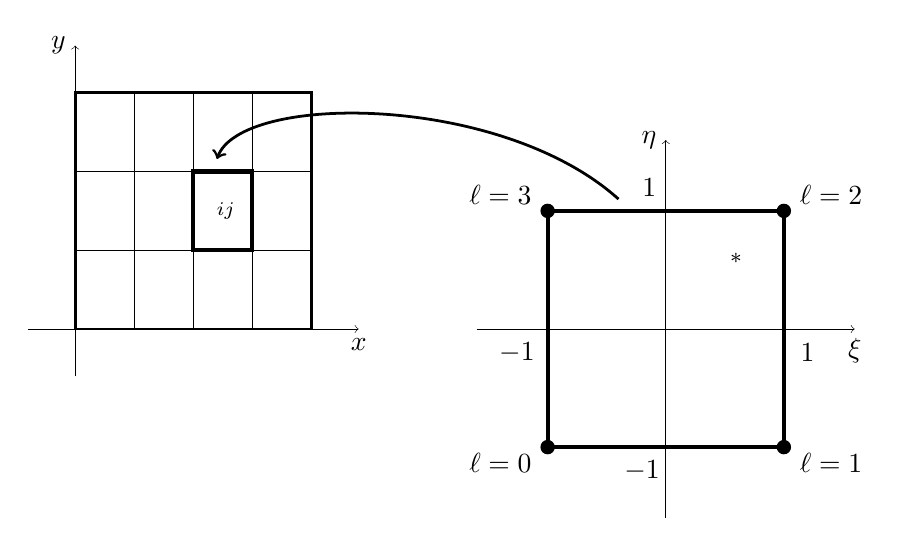
\begin{tikzpicture}[scale=3.0]
% (x,y) elements
  \draw[->,very thin] (-0.2,0.0) -- (1.2,0.0) node[below] {$x$};
  \draw[->,very thin] (0.0,-0.2) -- (0.0,1.2) node[left] {$y$};
  \draw[line width=1.0pt] (0.0,0.0) -- (0.0,1.0) -- (1.0,1.0) -- (1.0,0.0) -- cycle;
  \pgfmathsetmacro\fourth{1.0/4.0}
  \pgfmathsetmacro\third{1.0/3.0}
  \pgfmathsetmacro\twothird{2.0/3.0}
  \draw[xstep=\fourth,ystep=\third,black,thin] (0.0,0.0) grid (1.0,1.0);
  % outline an element
  \draw[line width=1.5pt] (0.5,\third) -- (0.75,\third) -- (0.75,\twothird) -- (0.5,\twothird) -- cycle;
  \node at (0.64,0.5) {$\square_{ij}$};

% (xi,eta) reference element
% origin of axes at (2.5,0.0) and square has half-width 0.5
  \draw[->,very thin] (1.7,0.0) -- (3.3,0.0) node[below] {$\xi$};
  \draw[->,very thin] (2.5,-0.8) -- (2.5,0.8) node[left] {$\eta$};
  \draw[line width=1.5pt] (2.0,-0.5) -- (3.0,-0.5) -- (3.0,0.5) -- (2.0,0.5) -- cycle;
  \node at (3.1,-0.1) {$1$};
  \node at (1.87,-0.1) {$-1$};
  \node at (2.43,0.6) {$1$};
  \node at (2.4,-0.6) {$-1$};
  \node at (2.8,0.3) {\large $\square_\ast$};
  \filldraw (2.0,-0.5) circle (0.8pt) node[xshift=-6mm,yshift=-2mm] {$\ell=0$};
  \filldraw (3.0,-0.5) circle (0.8pt) node[xshift=6mm,yshift=-2mm] {$\ell=1$};
  \filldraw (3.0,0.5) circle (0.8pt) node[xshift=6mm,yshift=2mm] {$\ell=2$};
  \filldraw (2.0,0.5) circle (0.8pt) node[xshift=-6mm,yshift=2mm] {$\ell=3$};

% arc
  \draw[->,line width=1.0pt] (2.3,0.55) .. controls (1.8,1.0) and (0.7,1.0) .. (0.6,0.72);
\end{tikzpicture}
\caption{Each element $\square_{ij}$ is the image under a map from the reference element $\square_\ast$.  The corners of $\square_\ast$ are numbered $\ell=0,1,2,3$.}
\label{fig:of:q1gridandref}
\end{figure}

The element map $\square_\ast \to \square_{ij}$ pictured in Figure \ref{fig:of:q1gridandref} can be written in either of two forms, the first\sidenote{The first form applies even in the case of logically-structured grids of quadrilaterals which are deformed in the $(x,y)$ plane, so-called \emph{isoparametric} finite elements \citep{Elmanetal2005}.} of which uses the above basis functions:
\begin{align}
x(\xi,\eta) &= \sum_{\ell=0}^3 x_\ell \chi_\ell(\xi,\eta) = x_i + \frac{h_x}{2} (1+\xi), \label{eq:of:referencemap} \\
y(\xi,\eta) &= \sum_{\ell=0}^3 y_\ell \chi_\ell(\xi,\eta) = y_j + \frac{h_y}{2} (1+\eta). \notag
\end{align}
The Jacobian of this map, used in integrals below, is the ratio of the area of $\square_{ij}$ to the area of $\square_\ast$:
\begin{equation}
\det\frac{\partial(x,y)}{\partial(\xi,\eta)} = \det\begin{bmatrix} \frac{h_x}{2} & 0 \\ 0 & \frac{h_y}{2} \end{bmatrix} = \frac{h_x h_y}{4}. \label{eq:of:elementjacobian}
\end{equation}

\begin{marginfigure}
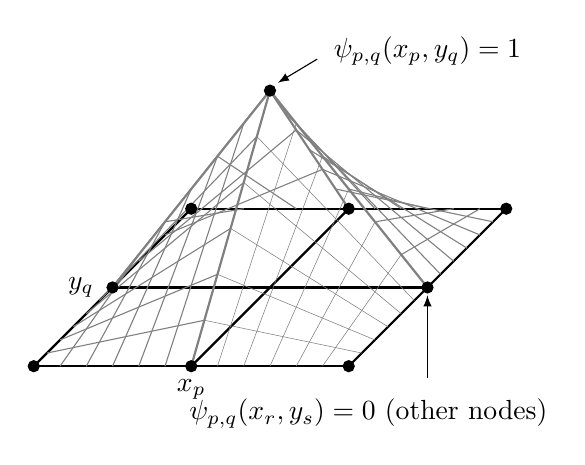
\begin{tikzpicture}[scale=0.5]

  % strong grid around elements
  \draw[thick] (0,0) -- (8,0);
  \draw[thick] (2,2) -- (10,2);
  \draw[thick] (4,4) -- (12,4);
  \draw[thick] (0,0) -- (4,4);
  \draw[thick] (4,0) -- (8,4);
  \draw[thick] (8,0) -- (12,4);

  \def\ytop{7};

  % tent lines
  \draw[gray,thick] (6,\ytop) -- (4,0);
  \draw[gray,thick] (6,\ytop) -- (2,2);
  \draw[gray,thick] (6,\ytop) -- (10,2);
  \draw[gray,thick] (6,\ytop) -- (8,4);

  \def\dx{(10.0-6.0)/6};
  \def\dy{(2.0-\ytop)/6};
  \foreach \jj in {1,...,5}
  {
       \draw[gray,very thin] ({6+\jj*\dx},{\ytop+\jj*\dy}) -- ({4+(4/6)*\jj},0.0);
  }

  \def\dx{(4.0-6.0)/6};
  \def\dy{(0.0-\ytop)/6};
  \foreach \jj in {1,...,5}
  {
       \draw[gray,very thin] ({6+\jj*\dx},{\ytop+\jj*\dy}) -- ({10-(2/6)*\jj},{2-(2/6)*\jj});
  }

  \def\dx{(2.0-6.0)/6};
  \def\dy{(2.0-\ytop)/6};
  \foreach \jj in {1,...,5}
  {
       \draw[gray,thin] ({6+\jj*\dx},{\ytop+\jj*\dy}) -- ({4-(4/6)*\jj},0.0);
  }

  \def\dx{(4.0-6.0)/6};
  \def\dy{(0.0-\ytop)/6};
  \foreach \jj in {1,...,5}
  {
       \draw[gray,thin] ({6+\jj*\dx},{\ytop+\jj*\dy}) -- ({2-(2/6)*\jj},{2-(2/6)*\jj});
  }

  \def\dx{(10.0-6.0)/6};
  \def\dy{(2.0-\ytop)/6};
  \foreach \jj in {1,...,5}
  {
       \draw[gray,thin] ({6+\jj*\dx},{\ytop+\jj*\dy}) -- ({8+(4/6)*\jj},4.0);
  }

  \def\dx{(8.0-6.0)/6};
  \def\dy{(4.0-\ytop)/6};
  \foreach \jj in {1,...,5}
  {
       \draw[gray,thin] ({6+\jj*\dx},{\ytop+\jj*\dy}) -- ({10+(2/6)*\jj},{2+(2/6)*\jj});
  }

  \def\dx{(2.0-6.0)/3};
  \def\dy{(2.0-\ytop)/3};
  \foreach \jj in {1,...,2}  % reduce clutter
  {
       \draw[gray,thin] ({6+\jj*\dx},{\ytop+\jj*\dy}) -- ({8-(4/3)*\jj},4.0);
  }

  \def\dx{(8.0-6.0)/3};
  \def\dy{(4.0-\ytop)/3};
  \foreach \jj in {1,...,2}
  {
       \draw[gray,thin] ({6+\jj*\dx},{\ytop+\jj*\dy}) -- ({2+(2/3)*\jj},{2+(2/3)*\jj});
  }

  % nodes in base plane
  \filldraw (0,0) circle (4pt);
  \filldraw (4,0) circle (4pt);
  \filldraw (8,0) circle (4pt);
  \filldraw (2,2) circle (4pt);
  %\filldraw (6,2) circle (4pt);   % (x_j,y_k) is at (6,2)
  \filldraw (10,2) circle (4pt);
  \filldraw (4,4) circle (4pt);
  \filldraw (8,4) circle (4pt);
  \filldraw (12,4) circle (4pt);

  % node at tent top
  \filldraw (6,\ytop) circle (4pt);

  % annotate
  \draw (10,\ytop+1.0) node {$\psi_{p,q}(x_p,y_q)=1$};
  \draw[-latex] (7.2,\ytop+0.8) -- (6.2,\ytop+0.2);
  \draw (8.5,-1.2) node {$\psi_{p,q}(x_r,y_s)=0$ (other nodes)};
  \draw[-latex] (10,-0.3) -- (10,1.8);

  % label center point
  \draw (4,-0.6) node {$x_p$};
  \draw (1.2,2) node {$y_q$};

\end{tikzpicture}

\caption{A hat function $\psi_{p,q} \in S^h$.}
\label{fig:of:q1hat}
\end{marginfigure}

For each node $(x_p,y_q)$ in the structured grid there is a continuous, piecewise-bilinear function $\psi_{p,q} \in S^h$, defined on all of $\overline\Omega$, which is equal to one on that node and equal to zero at all others:
\begin{equation}
  \psi_{p,q}(x_r,y_s) = \delta_{pr} \delta_{qs}.  \label{eq:of:psinodewise}
\end{equation}
Such ``hat'' functions, illustrated in Figure \ref{fig:of:q1hat}, form a basis of $S^h$.  When restricted to a particular element $\square_{ij}$ and pulled-back to the reference element $\square_\ast$, a hat function is either identically zero or it is equal to one of the basis functions $\chi_\ell$.  That is, if node $(\xi_\ell,\eta_\ell) \in \square_\ast$ corresponds to $(x_p,y_q)$ under the element map then 
\begin{equation}
  \psi_{p,q}(x(\xi,\eta),y(\xi,\eta)) = \chi_\ell(\xi,\eta)  \label{eq:of:phionref}
\end{equation}

To evaluate $I[u]$ in \eqref{eq:of:functional} we will want to compute gradients in the original $(x,y)$ variables.  Again in the case where $(\xi_\ell,\eta_\ell)$ and $(x_p,y_q)$ are identified by the element map, checking the following useful fact is an easy exercise:
\begin{equation}
  (\grad_{x,y} \psi_{p,q})(x(\xi,\eta),y(\xi,\eta)) = \left<\frac{2}{h_x}\frac{\partial\chi_\ell}{\partial \xi},\frac{2}{h_y}\frac{\partial\chi_\ell}{\partial \eta}\right>.   \label{eq:of:gradphionref}
\end{equation}
Derivatives $\partial\chi_\ell/\partial \xi$ and $\partial\chi_\ell/\partial \eta$ can be found from formula \eqref{eq:of:chidefn} above.

We are nearly ready to do the element-wise integrals in \eqref{eq:of:sumoverelements}, but at this point a summary is valuable and efficient.  Suppose we have $v \in S^h$.  Then it can be represented using the hat functions:
\begin{equation}
v(x,y) = \sum_{i=0}^{m_x-1} \sum_{j=0}^{m_y-1} v_{i,j} \psi_{i,j}(x,y)  \qquad \text{on } \,\Omega. \label{eq:of:bilinearrepresentation}
\end{equation}
This function is bilinear on element $\square_{i,j}$ and it pulls-back to the reference element $\square_\ast$, using the local node numbering, as
\begin{equation}
v(\xi,\eta) = \sum_{\ell=0}^3 v_\ell \chi_\ell(\xi,\eta)  \qquad \text{on } \,\square_\ast. \label{eq:of:bilinearref}
\end{equation}
The coefficient $v_\ell$ is equal to $v(x_r,y_s)$ for $(x_r,y_s)\in\square_{i,j}$ corresponding under the element map to $(\xi_\ell,\eta_\ell) \in \square_\ast$.  On the reference element the gradient has formula:
\begin{equation}
  (\grad_{x,y} v)(\xi,\eta) = \left<\frac{2}{h_x} \sum_{\ell=0}^3 v_\ell \frac{\partial\chi_\ell}{\partial \xi}, \frac{2}{h_y} \sum_{\ell=0}^3 v_\ell \frac{\partial\chi_\ell}{\partial \eta}\right>. \label{eq:of:gradrepref}
\end{equation}


\section{Quadrature}

We do not plan to do the integrals in \eqref{eq:of:sumoverelements} exactly, but instead by numerical integration (quadrature).  Indeed, for general $p>1$ it would be quite challenging to integrate the term ``$|\grad u|^p$'' exactly.

First we use change-of-variables to transfer the integral to the reference element.  Suppose $v(x,y)$ is any continuous function on element $\square_{i,j}$.  Using the element map and Jacobian formula \eqref{eq:of:elementjacobian} we have
\begin{align}
\int_{\square_{ij}} v(x,y)\,dx\,dy &= \int_{\square_\ast} v(\xi,\eta) \det\frac{\partial(x,y)}{\partial(\xi,\eta)}\,d\xi\,d\eta  \label{eq:of:changeofvars} \\
&= \frac{h_x h_y}{4} \int_{\square_\ast} v(\xi,\eta) \,d\xi\,d\eta \notag
\end{align}
where $v(\xi,\eta)=v(x(\xi,\eta),y(\xi,\eta))$.

FIXME in fact we only compute such integrals approximately by Gauss-Legendre

FIXME table with degree $n=1,2,3$ quadrature nodes $z_q$ and weights $w_q$ for integration over $[-1,1]$

FIXME tensor products for integrals over $\square_\ast$,
    $$\int_{\square_\ast} a(\xi,\eta) \,d\xi\,d\eta \approx \sum_{r=0}^n \sum_{s=0^n} w_r w_s a(z_r,z_s)$$


\clearpage
\newpage
\section{Implementation with objective only}

FIXME code uses \texttt{SNESSetObjective()} only, though also \texttt{SNESSetFunction()}; no hand-made Jacobian at all

FIXME try NCG

\cinputpart{plap.c}{\CODELOC}{FIXME I}{I}{//STARTCONFIGURE}{//ENDCONFIGURE}{code:plapI}

\cinputpart{plap.c}{\CODELOC}{FIXME II}{II}{//STARTEXACTF}{//ENDEXACTF}{code:plapII}

\cinputpart{plap.c}{\CODELOC}{FIXME III}{III}{//STARTOBJECTIVE}{//ENDOBJECTIVE}{code:plapIII}

\cinputpart{plap.c}{\CODELOC}{FIXME IV}{IV}{//STARTMAIN}{//ENDMAIN}{code:plapIV}


\section{Residual function $=$ gradient}

\cinputpart{plap.c}{\CODELOC}{FIXME V}{V}{//STARTFUNCTION}{//ENDFUNCTION}{code:plapV}


\section{Exercises}

\renewcommand{\labelenumi}{\arabic{chapter}.\arabic{enumi}\quad}
\renewcommand{\labelenumii}{(\alph{enumii})}
\begin{enumerate}
\item Prove coercivity \eqref{eq:of:coercivity} and convexity \eqref{eq:of:convexity} of functional $I[u]$ defined in \eqref{eq:of:functional}.  The finite dimensional facts that FIXME for $\xi,\eta\in\RR^n$ will be useful.

\item Show that $S^h$ is a linear subspace of $W^{1,p}(\Omega)$ with dimension $(m_x-1)(m_y-1)$.  What precisely is meant by saying $g$ is ``(appropriately) piece-wise linear on $\partial\Omega$'' in the definition of $S_g^h$ (page \pageref{eq:of:Sghdefn})?

\item  Use \eqref{eq:of:refcorners} and \eqref{eq:of:chidefn} to show that the two forms of the reference map \eqref{eq:of:referencemap} are the same.  Then use \eqref{eq:of:chidefn}, \eqref{eq:of:referencemap}, and \eqref{eq:of:phionref} to derive \eqref{eq:of:gradphionref}.

\item By testing against the integral
    $$\int_{\square_\ast} (1+\xi)^k + (1+\eta)^k\,d\xi\, d\eta = \frac{2^{k+3}}{k+1}$$
for $k=0,1,\dots,7$, confirm that the $n=1,2,3,4$ Gauss-Legendre quadrature formulas listed in the text will exactly integrate degree $2n-1$ degree polynomials, but not degree $2n$ polynomials, on the reference element.
% solution:  matlab/testgauss2d.m

\item FIXME
\end{enumerate}